% Copyright (C)  2015  Alexander Jankowski, Philipp Hacker.
% Permission is granted to copy, distribute and/or modify this document
% under the terms of the GNU Free Documentation License, Version 1.3
% or any later version published by the Free Software Foundation;
% with no Invariant Sections, no Front-Cover Texts, and no Back-Cover Texts.
% The lincense itself can be found at <https://www.gnu.org/licenses/fdl-1.3>.

\documentclass[numbers=noenddot,a4paper]{article}
%\documentclass[numbers=noenddot,12pt,a4paper,notitlepage,twoside,BCOR15mm]{scrartcl}

\usepackage[T1]{fontenc}
\usepackage[utf8]{inputenc}

\usepackage[infoshow]{tabularx}
\usepackage[all]{xy}

\usepackage{amsmath}
\usepackage{amssymb}
\usepackage{units}
\usepackage{upgreek}
\usepackage{esint}
\usepackage{graphicx}
\usepackage{ziffer}

\usepackage{float}
\usepackage{lscape}

\usepackage[labelfont=bf]{caption}
\usepackage{wrapfig}
\usepackage{subcaption}

\usepackage[backref=page]{hyperref}

\usepackage{csquotes}
\usepackage[infoshow]{tabularx}
\usepackage{fancyhdr}

\usepackage{sectsty}
\usepackage{times}

\usepackage{lmodern} %TODO Schriftart
\usepackage[english]{babel}
%\usepackage[greek,ngerman]{babel} %TODO Sprache einstellen

\renewcommand{\headrulewidth}{0.1pt}
\renewcommand{\footrulewidth}{0.1pt}
\newcommand{\name}{\text{}} %TODO Name des Protokollanten eintragen

\setlength{\parindent}{0pt}

\newcommand{\degree}{^\circ}
\newcommand{\diff}{\textnormal{d}}
\newcommand{\tenpo}[1]{ 10^{#1}}
\newcommand{\greek}[1]{\greektext#1\latintext}
\newcommand{\ix}[1]{_\text{#1}}
\newcommand{\imag}{\mathbf{i}}
\newcommand{\tilt}[1]{\textit{#1}}
\newcommand{\grad}[1]{\textit{grad}\left(#1\right)}
\newcommand{\divergenz}[1]{\textit{div}\left(#1\right)}
\newcommand{\euler}{\mathnormal{e}}
\newcommand{\fett}[1]{\textbf{#1}}
\newcommand{\ket}[1]{|#1\rangle}
\newcommand{\bra}[1]{\langle#1|}

\title{\fett{\underline{Protokoll: X-Ray
			Photoelectron Spectroskopy}}} %TODO Name des Versuchs eintragen
\author{Alexander Jankowski, Philipp Hacker}
\date{\today}
\pagestyle{fancy}
\fancyhead[C]{\thepage}
\fancyhead[R]{\name}
\fancyfoot[C]{\thepage}
\fancyhead[L]{Abschnitt \thesection}

\begin{document}

	\renewcommand*{\equationautorefname}{eq.}
	\renewcommand*{\figureautorefname}{fig.}
	\renewcommand*{\tableautorefname}{tab.}
	\renewcommand*{\sectionautorefname}{sec.}
	\renewcommand*{\subsectionautorefname}{sec.}
	\renewcommand*{\subsubsectionautorefname}{sec.}
	\renewcommand*{\figurename}{Fig. }
	\renewcommand*{\tablename}{Tab.}
	
	\renewcommand*{\figurename}{Figure }
	\renewcommand*{\tablename}{Table}


	\maketitle
\begin{center}
Supervisor: Dr. Robin John\\ %TODO Name des Betreuers eintragen
Date: 07.01.2016 \\ %TODO Datum des Versuchs eintragen
		\begin{table}[h]
	\centering
	Grade: %TODO Gute Note erhalten :)
			\begin{tabularx}{1.5cm}{|X|}
				\hline \\ \\
				\hline
			\end{tabularx}
		\end{table}
	\end{center}


	\vspace*{\fill}
	\tableofcontents
	\vfill
	\clearpage

	\section{Motivation}

The phenomena of the photoelectric effect is known since the beginning of the 20th century and lead to many methodes to examine surfaces of solid state bodies. One particual methode is the X-ray photoelectron spectroscopy or short \textbf{XPS}. It can give a good understanding of the composition of an solid state and furthermore it yields information about the chemical bounds between the different elements of the sample, effectively taking a fingerprint that can easily compared with similar samples. 

	\clearpage
	\section{Fundamentals}

To analyze the chemical and physical structure of a surface once can use photo electron spectroscopy (PES). For this high energetic electro magnetic radiation is applied to the surface. Due to this radiation the electrons bound to the atoms become excited and will be removed from the surface. In order to leave the solid body they have to overcome the binding energy $E_\mathrm{bin}$ and the work function $\phi$ and they will have a kinetic energy of
\begin{equation}
	E_\mathrm{kin} = h\nu - E_\mathrm{bin} - \phi,
\end{equation}
where $h \nu$ is the energy of the incitent photon. In order to release the electrons the photon energy has to be higher than the binding energy and the work function. Therefor high energetic X-Rays ($h\nu > 1000\mathrm\,{eV}$) will be used for the excitation. This methode is named X-Ray photoelectron spectroscopy (\textbf{XPS}).\\
Due to the different types of binding and the corresponding difference in binding energy, the released electrons have distinct kinetic energy, which makes it possible to determine the target material compsition and also the types of binding.
A closer look at the prosseses after the absorption of an pohoton by an elektron shows three stages in the prgress of the particle:
\begin{enumerate}
	\item The absoption of the ptoton and the excitation of the electron,
	\item The transport of the electron to the surface and
	\item The release of the electron followed by the detection.
\end{enumerate}

On the second stage the electrons can scatter and lose some of their momentum and therefore result in a background noice for the mesurement. 
Additionally to the specific peaks of the unscattered electron and the background one will notice peaks beneath the main peaks of one electronic state caused by small shifts in the binding energy due to the superposition of electronic and atomic states. This phenomena is called chemical shift and for this experiment, is mainly a result of oxidation of the surface.
In summary the Intensity of mesured electrons one yealds from the radiated sample can be expressed as

	\begin{align}
	I(E\ix{i},X\ix{i})=&I_{h\nu}T(E\ix{A})A_{\vartheta}\int_{\Omega=0}^{\Omega\ix{0}}\frac{\delta\sigma\ix{X}}{\delta\Omega}\diff \Omega\int_{0}^{d}D\ix{X}(z)\exp\left(-\frac{z}{\lambda\ix{mfp}sin(\vartheta)}\right)\diff z. \label{eq:intens} \\
	T(E\ix{A})&: \text{function of transmission of the apparatus} \nonumber\\
	A_{\vartheta}&: \text{adjusted surface of the sample towards the detector, at an solid angle } \Omega\, ,\,\,\vartheta \nonumber\\
	E\ix{i}&: \text{energy level i} \nonumber\\
	D\ix{X}(z)&: \text{density of electrons at the depth of the sample } z \nonumber\\
	\sigma\ix{X}&: \text{cross section of interaction between an electron at} E\ix{i}\, ,\,\, h\nu \nonumber
	\end{align}

Furthermore one has to consider, that the photons or more specificly the electrons that add to the detected yield, can vary strongly with the depth of the absorption of the photon or respectivly the the depth of the origin of the electron. X-ray-photons can penetrate the surface of a solid body by up to a few $\mathrm{\mu m}$, while the usual mean free path of an electron is  not more than a couple of $\mathbb{nm}$. That means that the deeper the electrons originates, the less unscattered electrons will be detected. The statistical relation according to  Lamber-Beer can be expressed as

	\begin{align}
	I\ix{e}(\lambda\ix{mfp})\propto\exp\left(-\frac{z}{\lambda\ix{mfp}}\right)\,\, .\label{eq:weg}
	\end{align}

In conclusion to that, a penetration depth $d \sim 3\lambda_\mathrm{mfp}$ can be defined, while the mean free path of the electron is dependent on its energy, its surroundings and the traveling direction. Experimental results for some metals and their penetration depth are shown in fig.\ref{fig:depth}

				\begin{figure}[h]
					\centering
					\fbox{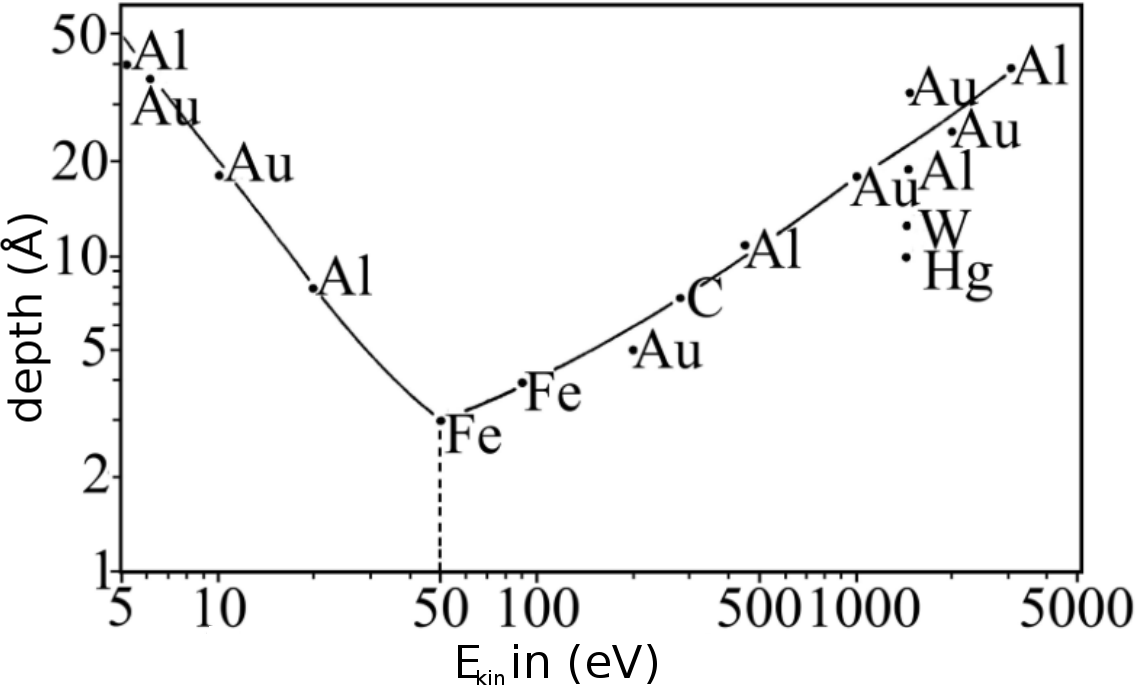
\includegraphics[width=0.75\textwidth]{pics/depth.png}}
					\caption{Exit depths of different metals over kinetic energy.\cite{XPSalt}}\label{fig:depth}
				\end{figure}
The mean free path can be expressed as

				\begin{align}
				\lambda\ix{mfp}=\frac{538\cdot a\unit{[nm]}}{(E\ix{kin}\unit{[eV]})^2}+0,41\cdot a^{3/2}\unit{[nm^{3/2}]}\sqrt{E\ix{kin}\unit{[eV]}} \,\,.\label{eq:mfp}
				\end{align}

Quantitative expressions about the composition can be achieved by the comparison of the peak areas $A_i$. One also has to consider different atomic sensitivity factors $ASF_i$ for the different elements.
In conclusion is the concentration of an element $i$ in an spectrum with multible elements $j$ given as followed
	\begin{align}
	c\ix{i}=\frac{A\ix{i}\cdot ASF\ix{i}^{-1}}{\sum_{j}A\ix{j}\cdot ASF\ix{j}^{-1}} \,\,.
	\label{eq:conc}
	\end{align}

	\clearpage
	\section{Realisation and Execution}

This experiment utilizes a vacuum chamber at a presure of approximitly \\ $10^{-8}\,\mathrm{mbar}$, which contains the rest of the aparatus, a x-ray tube with $\mathrm{Mg}$ as anode material, a fixure for the target with the ability to set the angle of incidence and an energy analysing detector for the secondary electorns. For the general messurement shown in fig.\ref{fig:aufbau} one uses the characteristic radiation of Magnesium $\mathrm{K\alpha}$ at a frequency of $1253\,\mathrm{eV}$. The incident radiation excites the bound electrons in the lower orbitals of the atoms. These electrons leave the atom with a distinct lower kinetic energy than the incident rations, since they need to overcome their binding energy. This distinct energy difference can be detected and will show up as peaks in the energy diagram. This typ of messurement is done multible times to compensate the statistical noice and also done with higher resolution for certain peaks in the spectrum ($\mathrm{O 1s, C 1s, Si 2p}$).

\begin{figure}[h]
	\centering
	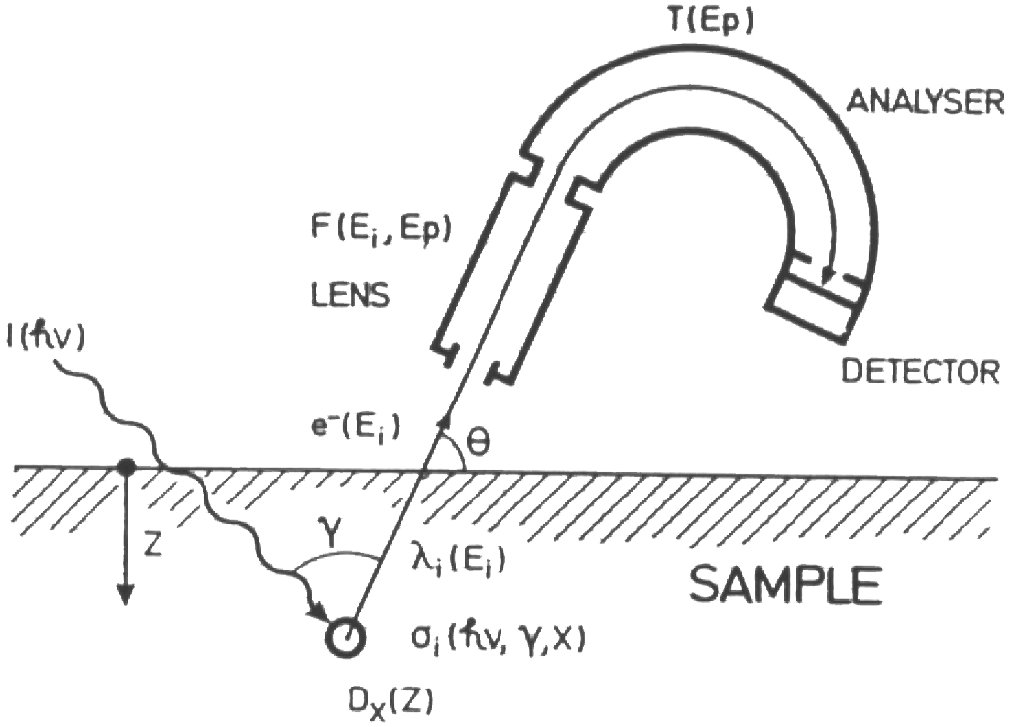
\includegraphics[width = 0.8 \columnwidth]{pics/aufbau.png}
	\caption{Schematic realization of the experiment.}
	\label{fig:aufbau}
\end{figure}

	\clearpage
	\section{Analysis}
	
	\subsection{Overview Spectrum}

The first mesurement consist of the making of a overview spectrum for the target witha an energy intervall of $100 - 1253\,\mathrm{eV}$ in steps of $0,5\,\mathrm{eV}$. To minimize the signal to noise ratio the mesurement is iterated over 10 cycles. The spectrum is shown in fig.\ref{fig:all}

				\begin{figure}[h]
					\centering
					\fbox{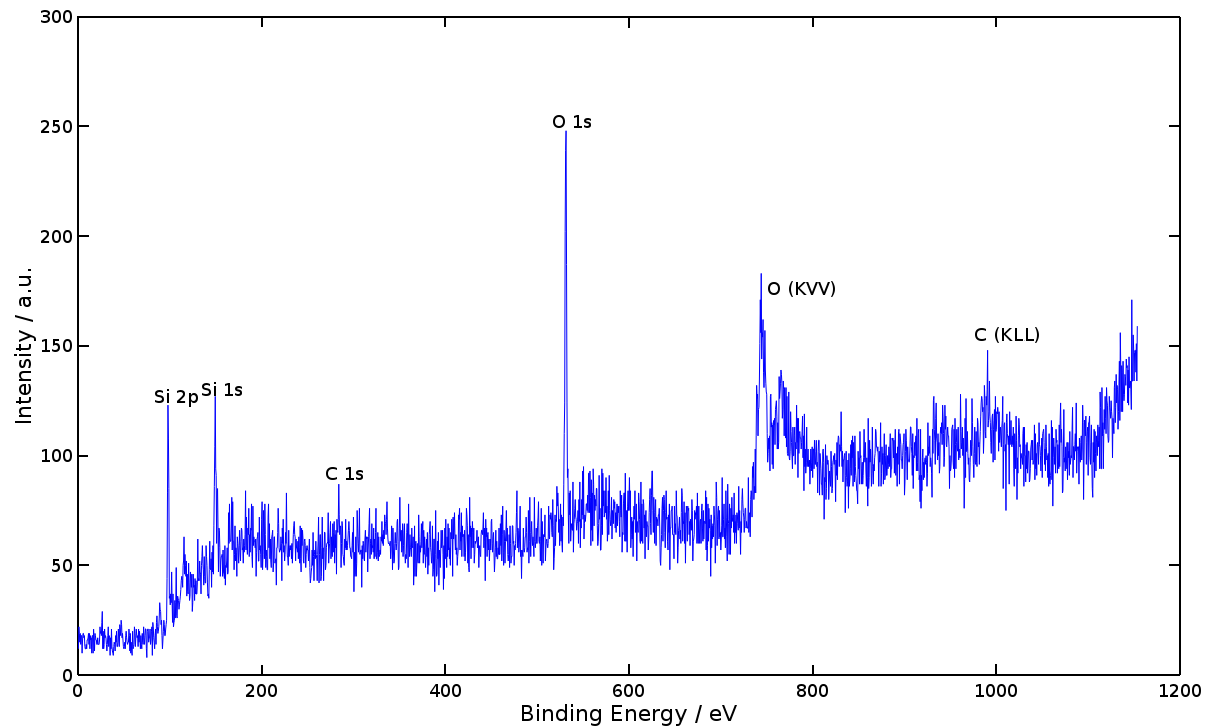
\includegraphics[width=1\textwidth]{pics/alles.png}}
					\caption{Overview spectrum of the Silicon target.}\label{fig:all}
				\end{figure}
The elements and nuclear niveaus corresponding to the energy peaks in the mesurement are matched with the the given data from the instruction manual. One distinctly notices, that the nuclear nievaus for Oxygen, Silicon and Carbon and the KLL-Auger-Lines and for Carbon and the KVV-Lines for Oxygen are matching the signal. Due to the limitations for the maximum energy given by the MgK$\alpha$-radiation higher nuclear levels and the Silicon-Auger-Lines can not observed in this spectrum.\\

\subsection{Single peaks}

In the following three of the peaks from the overview spectrum shall be examined more closely. For this, new mesurements are made in the respective energy intervalls at a higher resolution with 10 iterations per peak. The first peak is the $1s$ peak of Oxygen at $531,6\,\mathrm{eV}$ peak energy. The mesurement with a noise fit and gaussian fit is shown in fig.\ref{fig:O2}. The mesurement confirmes the expectations for the position of the peak.\\

\begin{figure}[t]
	\centering
	\fbox{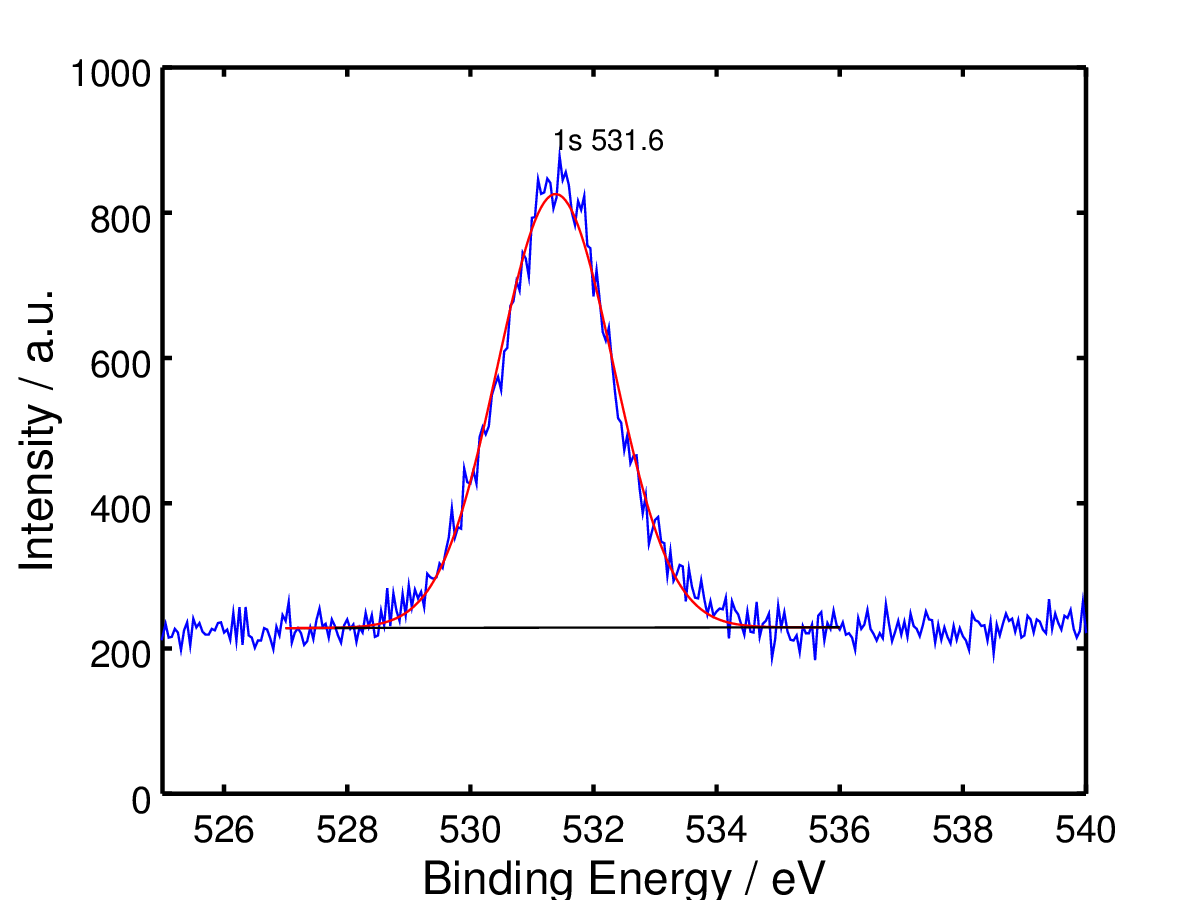
\includegraphics[width=0.65\textwidth]{pics/O1s.png}}
	\caption{Intensity of the photoelectron in an energyinterval near the O $1s$ binding energy. The blue line represents the mesured data, the black line represents a fit for the background noise and the  the drawn line red line represents a gaussian fit for the datapoints.}
	\label{fig:O2}
\end{figure}

The second peak is the $1s$ peak of Carbon. This peak is expected at an energy of $284,6\,\mathrm{ev}$ for polyethylene. The fig.\ref{fig:C1s} shows the mesured data with the background noise fit and the gaussian fit. In contrast to the Oxygen peak, this mesurement has a noticibly worse signal to noise ratio due to the relativly low yield for this peak.\\

\begin{figure}[!H]
	\centering
	\fbox{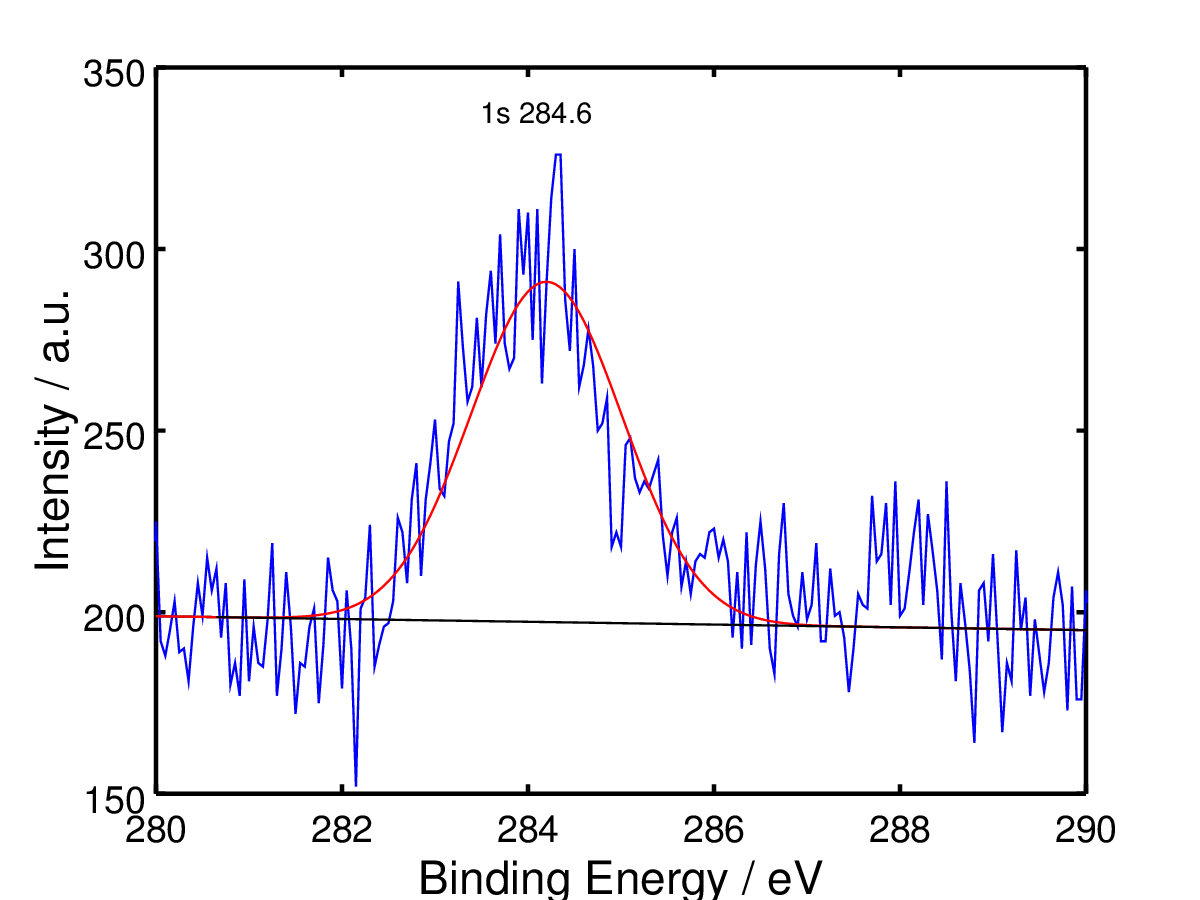
\includegraphics[width=0.65\textwidth]{pics/C1s.png}}
	\caption{Intensity of the photoelectron in an energyinterval near the C $1s$ binding energy. The blue line represents the mesured data, the black line represents a fit for the background noise and the  the drawn line red line represents a gaussian fit for the datapoints.}
	\label{fig:C1s}
\end{figure}

The third peak is the $2p$ peak of Silicon. The peak is expected at an energy of $99,15\,\mathrm{eV}$ with a secondary peak at $103,4\,\mathrm{eV}$ due to a chemical shift of Silicon bound in $\text{SiO}_2$. The Mesurement is shown in fig.\ref{fig:Si2p} with a background fit, two gaussian fit for the respective peaks and the combined value of the gaussian fits. The mesured data matches the expected position of the peaks.

\begin{figure}[!H]
	\centering
	\fbox{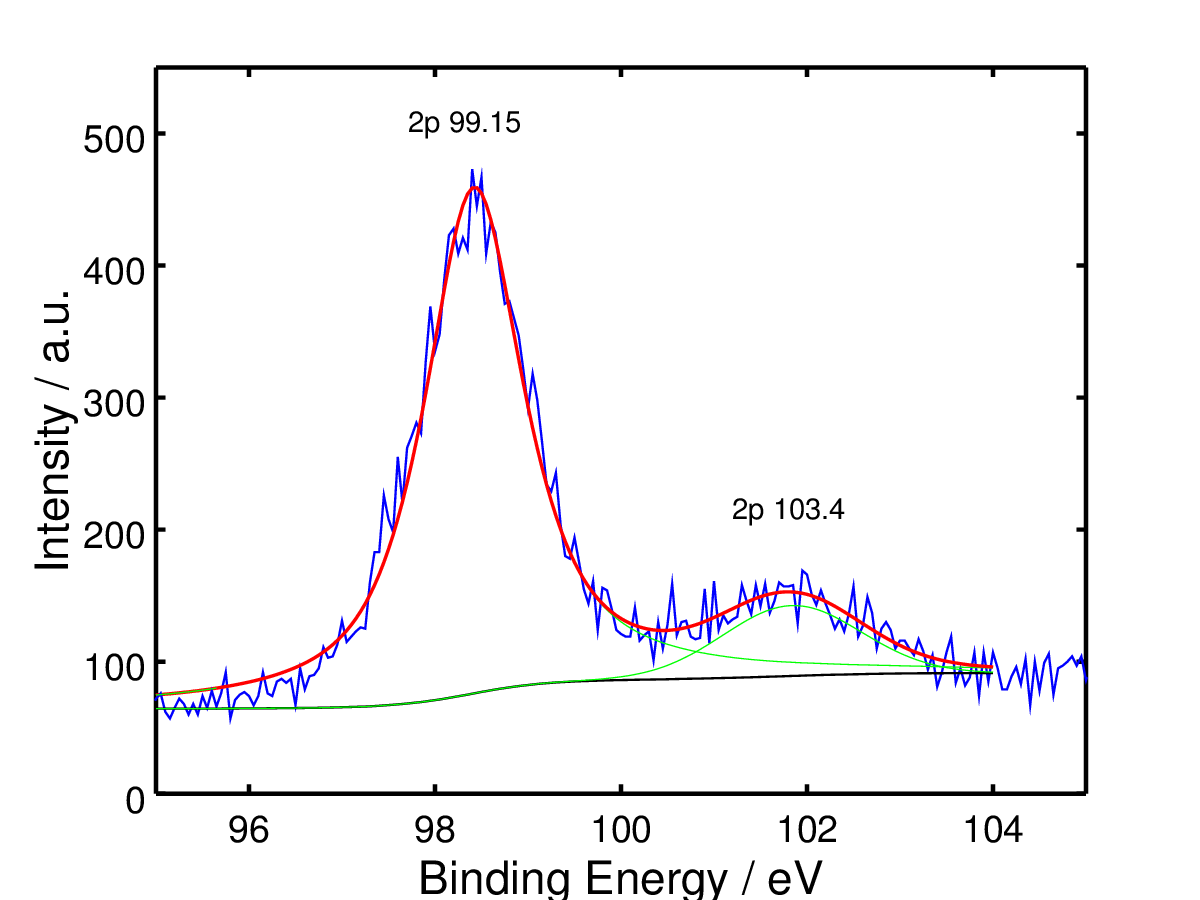
\includegraphics[width=0.65\textwidth]{pics/Si2p.png}}
	\caption{Intensity of the photoelectron in an energyinterval near the C $1s$ binding energy. The blue line represents the mesured data, the black line represents a fit for the background noise and the  the drawn line red line represents a gaussian fit for the datapoints.}
	\label{fig:Si2p}
\end{figure}



\subsection{Concentration of the Elements}

To determine the concentration of the mesured elements, once can use \eqref{eq:conc} and insert the area under the gaussian fit for $A$. The $ASF$ is taken from the instruction manual. The calculated concentrations are shown in tab.\ref{tab:conc}. The calculations impy, that the target consist of $42\%$ Silicon, where $6\%$ of that occurres in a bound with 2 Oxygen. Thus, one can assume, that $12\%$ of the Oxygen yield is bound to Silicon, where the remaining $27\%$ will be bound to the Carbon or other soiling.

\begin{table}[h]
	\centering
	\caption{Comparison of the different elements and their concentrations.}
	\begin{tabular}{c c r r r}
		\hline Element & Bondingstate & $A\,/\,\mathrm{a.u.}$ & $ASF$ & $c$ \\ \hline \hline
		O & 1s & $1384,83$ & $0,711$ & 0,39 \\ 
		C & 1s & $191,35$ & $0,296$ & 0,13 \\ 
		Si & 2p & $719,35$ & $0,339$ & 0,42 \\ 
		SiO$_2$ & 2p & $98.95$ & $0.339$ & 0,06 \\ \hline
	\end{tabular}
	\label{tab:conc}
\end{table}

	\clearpage
	\section{Apendix}

		\bibliography{all.bib}
		\bibliographystyle{unsrt}

\end{document}